Admins haben Zugriff auch besondere Funktionen um die Verwaltung im Frontend zu ermöglichen.
\paragraph{Nutzerverwaltung}~\\
Der nur als Admin einsehbare Menüpunkt ''Usermanagement'' führt auf die entsprechende Unterseite.\\
Hier kann ein Admin die registrierten User mit seiner UserId, sein Namen, seiner Email Adresse und der Anzahl der Playlisten/Videos einsehen (2) und folgende Funktionen nutzen:
\begin{itemize}
\item[(1)] Nach Usern suchen, dadurch kommt man auf eine Einzelansicht (5). Durch ein Suchen nach \texttt{:all} kommt man zurück zu allen Benutzern.
\item[(3)] Alle User außer Admins löschen
\item[(4)] Die User Gruppe von allen Usern außer Admins löschen
\end{itemize}
\begin{figure}[h!t]
\centering
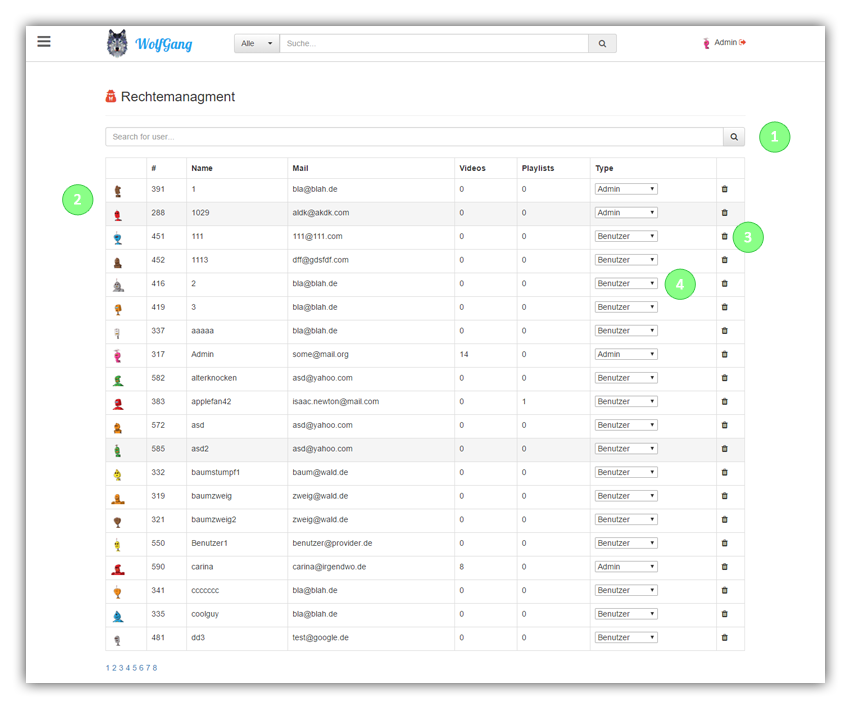
\includegraphics[width=\textwidth]{./Includes/Bedienungsanleitung/userma.png}
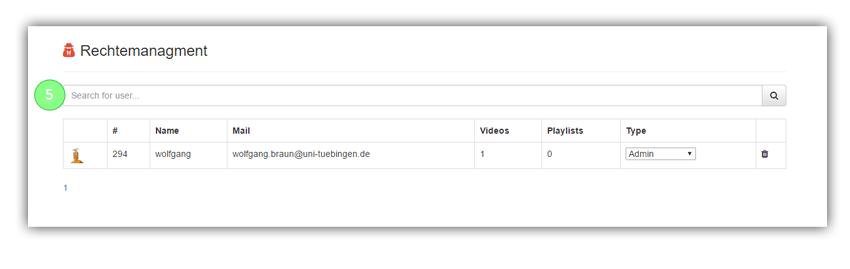
\includegraphics[width=\textwidth]{./Includes/Bedienungsanleitung/userma_search.png}
\end{figure}
\paragraph{Playlistverwaltung}~\\
Wenn ein Admin auf den Menüpunkt "Playlist" klickt, dann gelangt er statt zur normalen Useransicht, bei der Playlisten erstellt und angesehen werden können, zur Adminansicht, die zur Verwaltung der Playlisten verwendet wird (1). Neben einer Auflistung aller Playlisten werden folgende Funktionen zu Verfügung gestellt:
\begin{itemize}
\item[(2)] Der Name der Playlist geändert werden. Vergisst der Admin danach den Edit Knopf(3) zu drücken warnt ihn eine rote Umrandung vor
nicht gespeicherten Änderungen (4)
\item Jede Playlist kann gelöscht werden, egal wer sie erstellt hat (3)
\end{itemize}
\begin{figure}[h!t]
\centering
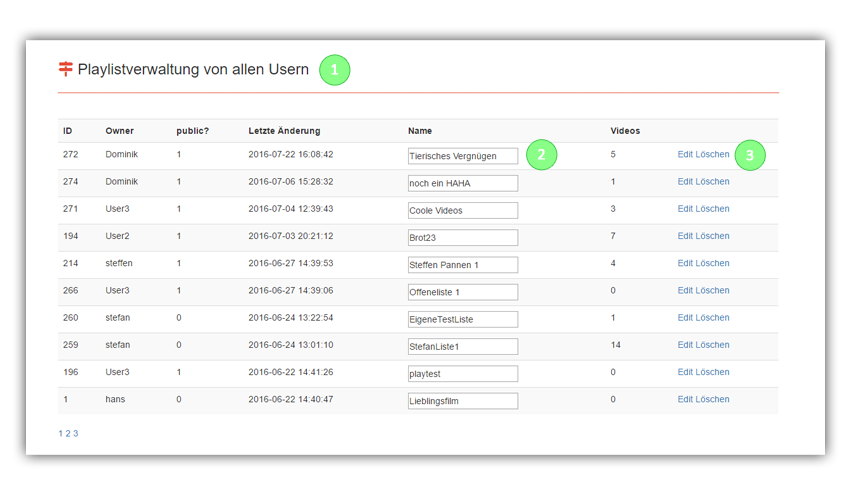
\includegraphics[width=\textwidth]{./Includes/Bedienungsanleitung/playlist_admin.png}
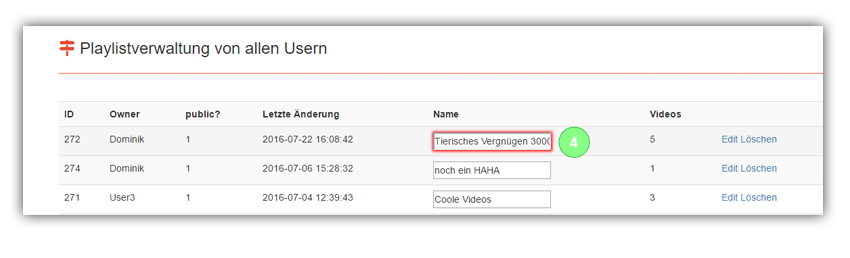
\includegraphics[width=\textwidth]{./Includes/Bedienungsanleitung/playlist_admin_edited.png}
\end{figure}
\paragraph{Kategorienverwaltung}~\\
Wenn ein Admin auf den Menüpunkt ''Kategorien'' klickt, erhält er ein leicht anderes Layout (1) als Nutzer der anderen Gruppen.\\
Hier wird die UserIds des Erstellers, der Name der Kategorie und die Anzahl der Videos angezeigt.\\
Außerdem kann ein Admin Kategorien umbenennen, löschen (3) und erstellen (2).
\begin{figure}[h!t]
\centering
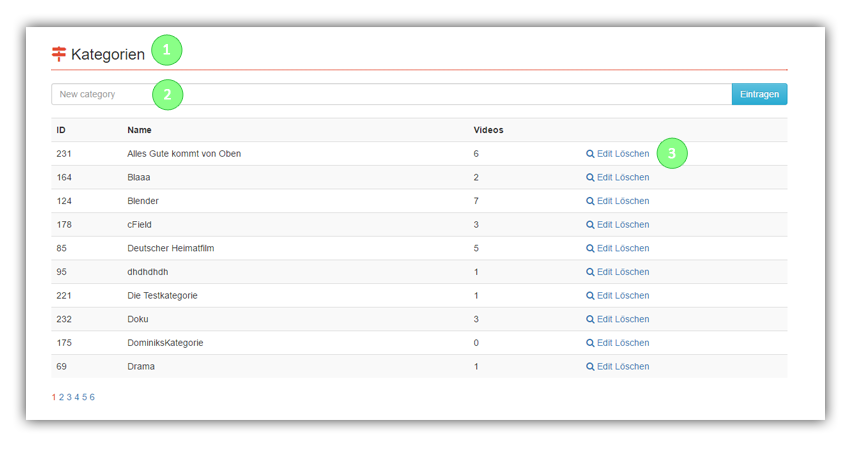
\includegraphics[width=\textwidth]{./Includes/Bedienungsanleitung/kategorien.png}
\end{figure}